\documentclass[12pt, titlepage]{article}

\usepackage{booktabs}
\usepackage{tabularx}
\usepackage{hyperref}
\usepackage{longtable}
\usepackage{array}
\usepackage{graphicx}
\usepackage{float}
\usepackage{color}
\graphicspath{ {img/} }

\hypersetup{
    colorlinks,
    citecolor=black,
    filecolor=black,
    linkcolor=red,
    urlcolor=blue
}
\usepackage[round]{natbib}

\title{SE 3XA3: Software Requirements Specification\\ReTouch}

\author{Team \#7, ReTouchers
		\\ Abrar Attia - attiaa1
		\\ Susan Fayez - fayezs
		\\ Mediha Munim - munimm
}


\begin{document}

\maketitle

\pagenumbering{roman}
\tableofcontents
\listoftables
\listoffigures

\begin{table}[bp]
\caption{\bf Revision History}
\begin{tabularx}{\textwidth}{p{3cm}p{2cm}X}
\toprule {\bf Date} & {\bf Version} & {\bf Notes}\\
\midrule
Oct 4 & 1.0 & Updated template with project/team names\\
Oct 5 & 1.1 & Added func. requirements and definitions \\
Oct 6 & 1.2 & Added project drivers and issues\\
Oct 6 & 1.3 & Added charts and work partitioning\\
Oct 6 & 1.4 & Added non-func. requirements \\
Oct 25 & 2.0 & Updated FREQ5 and FREQ15, updated list of terms \\
Oct 25 & 2.1 & Removed NFREQ4 , NFREQ17, and NFREQ23 \\
Oct 25 & 2.2 & Updated NFREQ10, NFREQ24, and NFREQ25\\
Oct 25 & 2.3 & Updated open issues and OTS solutions\\
Dec 4 & 3.0 & Updated use case diagram\\
Dec 4 & 3.1 & Added fit criteria to the non-functional requirements\\
Dec 4 & 3.2 & Prefixes for non-functional requirements updated\\
Dec 6 & 3.3 & Removed LF3\\
Dec 6 & 3.4 & Added FREQ16 and FREQ17\\

\bottomrule
\end{tabularx}
\end{table}

\newpage

\pagenumbering{arabic}

\section{Project Drivers}
\subsection{Purpose}
\indent \indent The purpose of this project is to re-implement the open source project K-Touch. K-Touch is a utility that allows users to track their speed and accuracy in typing, and results in improved typing skills through practice and repetition. The re-implementation will improve upon the original project by making it more user friendly and providing more comprehensive documentation.

\subsection{Stakeholders}
\indent \indent The stakeholders in this project are the clients, the developers, and the consumers. The clients are Dr. Bokhari and the TA's, as they are the ones who commissioned the project and it is their expectations that the developers are trying to meet. We, Abrar Attia, Mediha Munim, and Susan Fayez, are the developers of the project. The consumers or users for this project include any person who wishes to improve their typing skills.

\subsection{Mandated Constraints}
\indent \indent One of the main constraints for this project is the time frame in which it must be completed. The final prototype must be completed and demonstrated by November 27, 2017 and the final source code must be submitted by December 6, 2017.
\\
\indent Beyond time constraints, a major limiting factor for this project is that it must have similar functionality to the original K-Touch project. It must offer various text "lessons" for the user to type as quickly and as accurately as they can while offering real-time statistics on their accuracy and speed. 
\\
\indent The functionality of the actual program will be constrained by the speed and processing power of the computer on which it is run. This is an issue that is present with the original project, as the program experiences heavy delays between the user input and the interface response.


\subsection{Naming Conventions and Terminology}

\begin{itemize}
    \item \textbf{Lessons:} The selections of text provided by the application for the user to type as quickly and accurately as they can.
    \item \textbf{K-Touch:} The original project. A utility that is designed to help users improve their typing skills.
    \item\textbf{Completed character:} A character is completed if the user has successfully typed it on the keyboard when it was the current character. 
    \item \textbf{Current character:} The character that the user is expected to input at a given moment.
    \item\textbf{Incorrect character:} A character is incorrect if the wrong keyboard character was inputted by the user when it had been the current character.
    \item\textbf{Noncompleted character:} A character is noncompleted if it is not a completed character.
    \item \textbf{Lesson beginning:} The moment when the list of words is first generated and displayed on screen.
    \item \textbf{Lesson end:} The moment when the last character in the current list of words has been completed.
    \item \textbf{Results}: {\color{cyan}The time, typing accuracy, and typing speed of the user calculated at the end of a lesson.}
\end{itemize}

\subsection{Relevant Facts and Assumptions}
\indent \indent The original project comes with very little user instruction and often experiences heavy delays between the user input and the interface's representation of the user's progress. It also has an unfair policy of requiring the user to type with 100\% accuracy in order to advance progress in the lesson. These are issues that need to be addressed in the re-implementation.
\\
\indent The project will be implemented in such a way that it is assumed that the user has basic knowledge of computers, enough to open and run the program. Beyond that, the project will be user friendly and provide comprehensive instructions to ensure the user has an optimal experience. It will also be assumed that the program will be used by one user at a time on a desktop or laptop computer with a physical keyboard.

\section{Functional Requirements}

\subsection{The Scope of the Work and the Product}

\subsubsection{The Context of the Work}

\begin{figure}[h!]
	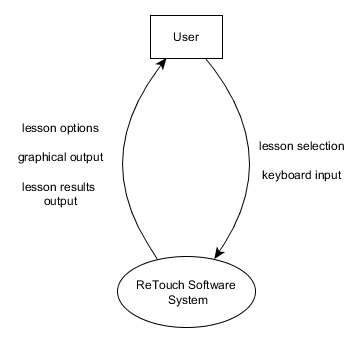
\includegraphics[scale=0.75]{ContextDiagram.jpg}
	\centering
	\label{figure:1}	
	\caption{The context diagram for ReTouch.}
\end{figure}

\subsubsection{Work Partitioning}

\begin{table}[H]
  \caption{The work partitioning for ReTouch.}
\begin{tabular}{ |m{2.5cm}|m{3cm}|m{7cm}| }

    \hline
    \textbf{Event Name} & \textbf{Input/Output} & \textbf{Summary} \\ 
    \hline
    Lesson\newline Selection & OUTPUT: List of lessons \newline INPUT: User-specified lesson & The user chooses a lesson from those available on screen. \\
    \hline
    Keyboard & INPUT: Keyboard input & The user's input, consisting of the characters that the user types in.  \\
    \hline
    Graphical\newline Output & OUTPUT: Characters to be typed, real-time user information & The system outputs the GUI, consisting of the characters that need to be typed, as well as the user's current typing speed, accuracy, and timing. \\
    \hline
    Lesson\newline Results & OUTPUT: User's typing information. & The system outputs the user's overall typing speed, accuracy, and timing data gathered from the completion of the lesson by displaying it on the screen. \\
    \hline

\end{tabular}
\end{table}

\subsubsection{{\color{cyan}Use Cases}}

\begin{figure}[H]
	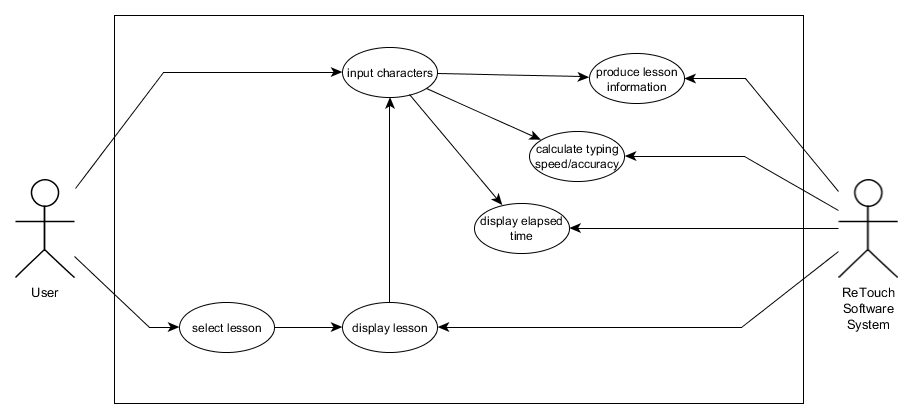
\includegraphics[scale=0.4]{UseCaseDiagram.jpg}
	\centering
	\label{figure:2}	
	\caption{The use cases for ReTouch.}
\end{figure}

\subsection{Functional Requirements}

\begin{longtable}{ |m{2cm}|m{1.8cm}|m{9.4cm}| }
\caption{The functional requirements for ReTouch.} \\
    \hline
    \textbf{Identifier} & \textbf{Priority} & \textbf{Requirement} \\ 
    \hline
    FREQ1 & 2 & The system should allow the user to choose between various lessons, each lesson consisting of a different combination of keyboard symbols/letters. \\ 
    \hline
    FREQ2 & 5 & The system shall generate a list of characters consisting of the specified letter/symbol combinations. The list shall consist of less than \hyperref[symbols]{MAX\_LESSON} characters, including spaces. \\ 
    \hline
    FREQ3 & 5 & The system shall display the list of characters using the specified character combinations for the user to type up. The list of characters will be presented on separate lines, with each line being no greater than constant \hyperref[symbols]{MAX\_LINE}.  \\ 
    \hline
    FREQ4 & 5 & The system shall begin the program at the first character (which will become the current character) and wait for the user to type a character. \\ 
    \hline
    FREQ5 & 5 & {\color{cyan}The system shall move the current character to the next character (to the right) when the user inputs a character (incorrect or not), unless the current character is at the end of a line. If it is at the end of a line, the current character will not change. }  \\ 
    \hline
    FREQ6 & 5 & The system shall set a current character as completed if the user presses the same character that is indicated by the current character. \\ 
    \hline
    FREQ7 & 4 & The system shall indicate when an incorrect character has been typed by highlighting the incorrect character. All characters typed after an incorrect character will be considered incorrect, and highlighted as well. \\ 
    \hline
    FREQ8 & 4 & The system shall allow the user to move on to the next line only when they have reached the last character on the current line and all the characters on the line are correct. When the “ENTER” key is pressed, the current character will become the first character on the next line. \\ 
    \hline
    FREQ9 & 4 & The system shall remove the character to the left of the current character and move the current character to the left when the “BACKSPACE” key is pressed. However, if the current character is the first character of a line, nothing will happen when “BACKSPACE” is pressed. \\ 
    \hline
    FREQ10 & 2 & The system should count the number of times an incorrect character is typed. \\ 
    \hline
    FREQ11 & 2 & The system should display the elapsed time from when a lesson begins to when the lesson is completed. \\ 
    \hline
    FREQ12 & 2 & The system should display the typing accuracy of the user. \\ 
    \hline
    FREQ13 & 2 & The system should display the typing speed of the user. \\ 
    \hline
    FREQ14 & 4 & The system shall end the typing lesson when all characters are completed and “ENTER” is pressed. \\ 
    \hline
    FREQ15 & 3 & {\color{cyan}The system should display the results of the lesson after the lesson is done. }\\ 
    \hline
    \color{cyan}FREQ16 & \color{cyan} 3 & {\color{cyan}The system should allow the user to return to the lesson selection page during a lesson. }\\
    \hline
    \color{cyan}FREQ17 & \color{cyan} 3 & {\color{cyan}The system should allow the user to return to the lesson selection page at the lesson results page. }\\
    \hline

\end{longtable}

\section{Non-functional Requirements}
\subsection{Look and Feel Requirements}

\begin{table}[H]
  \caption{The look and feel requirements for ReTouch.}
\begin{tabular}{ |m{2cm}|m{1.8cm}|m{9.4cm}| }
    \hline
    \textbf{Identifier} & \textbf{Priority} & \textbf{Requirement} \\ 
    \hline
    {\color{cyan}LF1} & 5 & The application will open to an introductory page that has multiple lesson options displayed. \\ 
    \hline
    {\color{cyan}LF2} & 5 & Once the lesson begins, the application will display all the required characters for the lesson in a text box. The current character will be highlighted to notify the user on what character to enter next. \\ 
    \hline
    {\color{cyan}LF3} & 3 & The GUI's components will be consistent in colour, text fonts, and window properties in order to keep the application organized and easy to navigate. \\ 
    \hline
\end{tabular}
\end{table}

\subsection{Usability and Humanity Requirements}

\begin{table}[H]
  \caption{The usability and humanity requirements for ReTouch.}
\begin{tabular}{ |m{2cm}|m{1.8cm}|m{9.4cm}| }
    \hline
    \textbf{Identifier} & \textbf{Priority} & \textbf{Requirement} \\ 
    \hline
    {\color{cyan}UH1} & 5 & The application interface will be easy to use for any individual who is able to use a computer and keyboard and requires typing practice. {\color{cyan}The user should be able to navigate all three pages without instruction}\\
    \hline
    {\color{cyan}UH2} & 5 & The application will be easy to follow and will not require any additional training to use. {\color{cyan}The user should be able to complete the lesson without instruction}\\ 
    \hline
    {\color{cyan}UH3} & 4 & The application will provide typing lessons that appeal and work for individuals who are beginners with typing, people who are considered experts and can type proficiently, and everyone in between. {\color{cyan}There should be at least one lesson that the user finds challenging.}\\
    \hline
    {\color{cyan}UH4} & 4 & The application will be easy to install by any user. {\color{cyan}The user should be able to run the program with the provided instructions.}\\
    \hline
\end{tabular}
\end{table}

\subsection{Performance Requirements}

\begin{table}[H]
  \caption{The performance requirements for ReTouch.}
\begin{tabular}{ |m{2cm}|m{1.8cm}|m{9.4cm}| }
    \hline
    \textbf{Identifier} & \textbf{Priority} & \textbf{Requirement} \\ 
    \hline
    {\color{cyan}P1} & 5 & {\color{cyan}The application will respond to user input within 1 second. Furthermore, every completed character inputted by the user will allow the application to move to the next character.} \\
    \hline
    {\color{cyan}P2} & 5 & The applications recorded elapsed time will be accurate and begin right when the lesson loads and will stop when the user presses “ENTER”. {\color{cyan}This should be apparent from the GUI }\\ 
    \hline
    {\color{cyan}P3} & 4 & The application will be reliable and will only fail or crash in extreme unexpected circumstances. \\
    \hline
    {\color{cyan}P4} & 4 & The application will be a single-user system. \\
    \hline
    {\color{cyan}P5} & 4 & The application will not interfere with the user's machine. \\
    \hline
\end{tabular}
\end{table}

\subsection{Operational and Environmental Requirements}

\begin{table}[H]
  \caption{The operational and environmental requirements for ReTouch.}
\begin{tabular}{ |m{2cm}|m{1.8cm}|m{9.4cm}| }
    \hline
    \textbf{Identifier} & \textbf{Priority} & \textbf{Requirement} \\ 
    \hline
    {\color{cyan}OE1} & 4 & The application will be functional in Windows, {\color{cyan}Mac,} and Linux. \\
    \hline
    {\color{cyan}OE2} & 4 & The application will not depend on any other partner applications. \\
    \hline
\end{tabular}
\end{table}

\subsection{Maintainability and Support Requirements}

\begin{table}[H]
  \caption{The maintainability and support requirements for ReTouch.}
\begin{tabular}{ |m{2cm}|m{1.8cm}|m{9.4cm}| }
    \hline
    \textbf{Identifier} & \textbf{Priority} & \textbf{Requirement} \\ 
    \hline
    {\color{cyan}M1} & 3 & The source code of the application will be open to the public. \\
    \hline
\end{tabular}
\end{table}

\subsection{Security Requirements}

\begin{table}[H]
  \caption{The security requirements for ReTouch.}
\begin{tabular}{ |m{2cm}|m{1.8cm}|m{9.4cm}| }
    \hline
    \textbf{Identifier} & \textbf{Priority} & \textbf{Requirement} \\ 
    \hline
    {\color{cyan}S1} & 4 & The application will remain confidential and will not store user results.\\
    \hline
    {\color{cyan}S2} & 4 & The applications source code will not be augmented by any changes or updates made by the user when using the application. \\
    \hline
\end{tabular}
\end{table}

\subsection{Cultural Requirements}

\begin{table}[H]
  \caption{The cultural requirements for ReTouch.}
\begin{tabular}{ |m{2cm}|m{1.8cm}|m{9.4cm}| }
    \hline
    \textbf{Identifier} & \textbf{Priority} & \textbf{Requirement} \\ 
    \hline
    {\color{cyan}C1} & 3 & The application shall not be offensive in any way to any potential user.\\
    \hline
    {\color{cyan}C2} & 3 & All the text within the application will be available in English. \\
    \hline
\end{tabular}
\end{table}

\subsection{Legal Requirements}

{\color{cyan}No legal requirements at this time.}

\subsection{Health and Safety Requirements}

\begin{table}[H]
  \caption{The health and safety requirements for ReTouch.}
\begin{tabular}{ |m{2cm}|m{1.8cm}|m{9.4cm}| }
    \hline
    \textbf{Identifier} & \textbf{Priority} & \textbf{Requirement} \\ 
    \hline
    {\color{cyan}HS1} & 3 & {\color{cyan}The application shall not impose any health risks upon its users. For instance, there will be no extreme flashing lights that may impact users with epilepsy. }\\
    \hline
     {\color{cyan}HS2} & 3 & {\color{cyan}A warning shall be placed in the instructions that extreme repetitive usage of the application that could cause strain on muscles and eyes.} \\
    \hline
    {\color{cyan}HS3} & 3 & {\color{cyan}The application shall not impose any safety risks upon its users. For instance, the users information will not be made public.} \\
    \hline
\end{tabular}
\end{table}

\section{Project Issues}
\subsection{Open Issues}
\indent \indent In the re-implementation of this project, the source code will be converted from C/C++ to Java. This presents several issues, the most critical of which being the use of required libraries. These libraries may not be portable to Java, which could hinder the functionality of our implementation. 
\\
\indent Another challenge this project faces is the lack of familiarity the developers have with the language the original project is implemented in. One group member has limited knowledge of C/C++, but it will still be problematic for the developers to understand the original source code enough to re-implement and improve upon it.
\\
\indent Similarly, the developers of this project have never worked on a project of this scope. It will be a challenge to ensure that each component of the application runs smoothly, accurately, and concurrently.

\indent {\color{cyan}The project itself also has issues that can be improved upon. The project we are basing our implementation on runs only on Linux, meaning portability can be greatly improved upon. Additionally, this application only has single user functionality, missing out on the benefits that a competitive element may bring to the user. By putting them against other users, they may be further motivated to improve their performance.}

\subsection{Off-the-Shelf Solutions}
\indent \indent {\color{cyan}Many similar applications to K-Touch exist that are readily available to users. There are competitive online applications that allow users to race others to accurately complete a selection of text, such as TypeRacer, FreeTypingGame, Nitro Type, and Rapid Typing. These applications solve the competitiveness issue. There are also applications that are more similar to K-Touch, in that they focus singularly on the user and helping them improve their speed and accuracy, such as Typng Master, Key Hero, and 10FastFingers. All of the mentioned applications are available online, solving the portability issue.}

\subsection{New Problems}
\indent \indent The use of this application can potentially cause new problems for the user. One such problem is a potential Repetitive Strain Injury such as Carpal Tunnel Syndrome if the application is used for a prolonged period of time in a non-ergonomic way. 

\subsection{Tasks}
\indent \indent The tasks for this project are essentially to complete the deliverables prescribed by Dr. Bokhari within the time frame he provides. The final code should be completed by November 27, 2017 for the final demonstration. Other deliverables include: the Problem Statement, Development Plan, Requirements Document, Proof of Concept Demonstration, Test Plan, Design Document, Revision 0 Demonstration, Peer Evaluation, Test Plan, Test Report, and User Guide.

\subsection{Risks}
\indent \indent The biggest risk for this project is that the developers may be too unfamiliar with aspects of the original project to effectively re-implement it. Given the time constraints on the project, they must learn quickly in order to have a viable product at the end of the project term. Another risk is in the conversion from C/C++ to Java. It is possible the new project won't be able to have the same level of functionality as the original in the transition.

\subsection{Costs}
\indent \indent The cost for this project will simply be the time and energy of the developers. They will invest their energy in coding, learning elements of C/C++, researching libraries, learning how to develop GUI's, potentially learning how to implement wrappers, writing documentation, and presenting their work.

\subsection{User Documentation and Training}
\indent \indent The final application shall be very user-friendly and easy to use. Comprehensive instructions will be included to diminish any chance of uncertainty in using the product.

\subsection{Ideas for Solutions}
\indent \indent For the issue of having incompatible required libraries, the first solution would be to search for libraries in Java that have the same functionality as the original C/C++ libraries. Should this solution fail and no viable Java libraries are found, the next solution would be to implement a wrapper for the original libraries to make them usable in Java.

\indent For the issues of inexperience and unfamiliarity, the solution is for the developers to commit themselves to researching and learning about the areas in which they are unclear. Online resources and the help of TA's will be implemented when needed.

\newpage

\subsection{Symbolic Parameters} \label{symbols}

\begin{itemize}
\item MAX\_LESSON: The maximum number of characters per lesson.
\item MAX\_LINE: The maximum number of characters per line.
\end{itemize}


\end{document}

